\section{Bài 4}

\subsection{Đề bài}

Cài đặt hoàn chỉnh thuật toán Grover và thực hiện các tính toán cho thấy hoạt động của thuật toán khi lời giải là $0^n$ trong trường hợp $n=4$. Kiểm tra kết quả trên thư viện Qiskit.

\subsection{Lời giải}

Dưới đây là mã nguồn Python sử dụng Qiskit để cài đặt thuật toán Grover với lời giải là $\ket{0000}$ cho $n=4$ qubit. Thuật toán sẽ được lặp lại 3 lần để khuếch đại xác suất đo được trạng thái mục tiêu.
\begin{lstlisting}[language=Python]
def initialize_s(qc, n):
    """Create equal superposition state |s>"""
    qc.h(range(n))


def oracle_0000(qc, n):
    """
    Oracle marking |0000>
    X - MCP(pi) - X
    """
    qc.x(range(n))
    qc.mcp(np.pi, list(range(n - 1)), n - 1)
    qc.x(range(n))


def diffuser(qc, n):
    """
    Diffuser operator
    """
    qc.h(range(n))
    qc.x(range(n))
    qc.mcp(np.pi, list(range(n - 1)), n - 1)
    qc.x(range(n))
    qc.h(range(n))


n = 4  # number of qubits
qc = QuantumCircuit(n)

initialize_s(qc, n)
qc.barrier()

iterations = 3
for i in range(iterations):
    oracle_0000(qc, n)
    qc.barrier()
    diffuser(qc, n)
    qc.barrier()

qc.measure_all()

simulator = AerSimulator()
compiled_circuit = transpile(qc, simulator)
result = simulator.run(compiled_circuit, shots=1024).result()
counts = result.get_counts()

print(f"Simulation results for n={n}, Target=|0000> after {iterations} iterations:")
sorted_counts = dict(sorted(counts.items(), key=lambda item: item[1], reverse=True))
print(sorted_counts)

plot_histogram(counts)
\end{lstlisting}

Kết quả của mô phỏng trên:
\begin{lstlisting}
Simulation results for n=4, Target=|0000> after 3 iterations:
{'0000': 979, '0111': 7, '0100': 5, '0010': 5, '1110': 5, '1001': 4, '0001': 4, '1111': 3, '1100': 2, '0101': 2, '1000': 2, '0110': 2, '0011': 1, '1011': 1, '1101': 1, '1010': 1}
\end{lstlisting}

\begin{figure}[H]
    \centering
    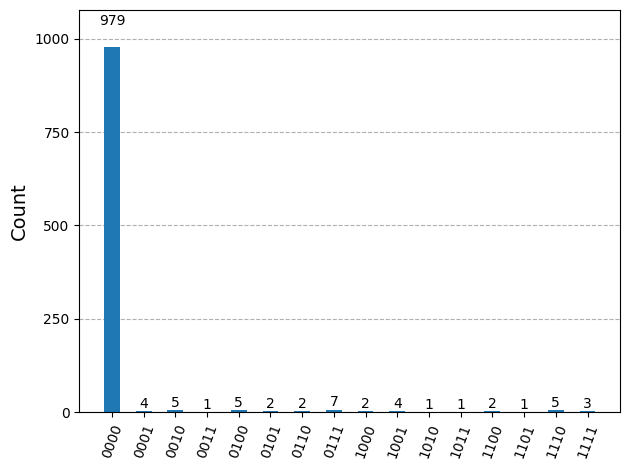
\includegraphics[width=0.6\textwidth]{img/section4_results.png}
    \caption{Thống kê kết quả mô phỏng thuật toán Grover với lời giải là $\ket{0000}$ cho $n=4$ qubit sau 3 lần lặp.}
    \label{fig:hw4_grover_histogram}
\end{figure}